\chapter{\ploren{Część praktyczna}{Implementation and results}}

Tutaj powinien znaleźć się opis własnego rozwiązania, stanowiska, implementacji oraz wyników badań lub testów. Dla elektrotechniki może to być projekt i pomiary układu lub urządzenia; dla automatyki identyfikacja obiektu, projekt regulatora i eksperyment; dla informatyki architektura, implementacja oraz ocena jakości, wydajności lub bezpieczeństwa systemu.

\section{\ploren{Obiekt badań lub projektowane rozwiązanie}{Research object or designed solution}}

\section{\ploren{Stanowisko i środowisko badawcze}{Test bench and research environment}}

\section{\ploren{Metodyka i przebieg badań}{Research methodology and procedure}}

\section{\ploren{Wyniki, analiza niepewności i dyskusja}{Results, uncertainty analysis and discussion}}

Przykładowy wykres funkcji kwadratowej przedstawiono na rysunku \ref{fig:wykres-kwadratowej}. Dla funkcji
\(f(x)=x^2-2x-3\) parabola jest skierowana ramionami do góry, a jej wierzchołek znajduje się w punkcie
\((1,-4)\).

\begin{figure}[!ht]
  \centering
  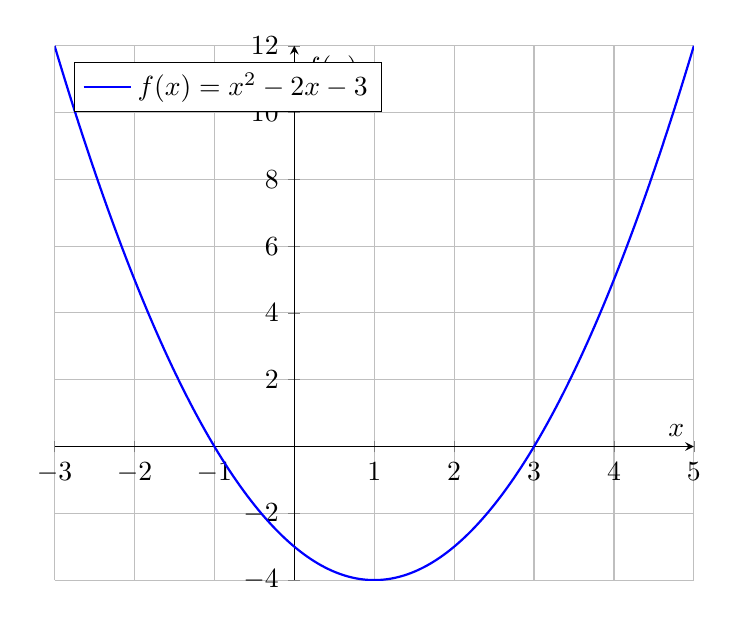
\begin{tikzpicture}
    \begin{axis}[
      width=0.8\textwidth,
      xlabel={$x$},
      ylabel={$f(x)$},
      grid=both,
      domain=-3:5,
      samples=200,
      axis lines=middle,
      legend pos=north west
    ]
      \addplot[thick, blue] {x^2 - 2*x - 3};
      \addlegendentry{$f(x)=x^2-2x-3$}
    \end{axis}
  \end{tikzpicture}
  \caption{Przykładowy wykres funkcji kwadratowej}
  \label{fig:wykres-kwadratowej}
\end{figure}

Przykładowy wykres słupkowy funkcji pierwiastkowej przedstawiono na rysunku \ref{fig:wykres-slupkowy-pierwiastkowej}. Dla funkcji
\(g(x)=\sqrt{x}\) wartości rosną wraz ze wzrostem argumentu, jednak tempo tego wzrostu stopniowo maleje.

\begin{figure}[!ht]
  \centering
  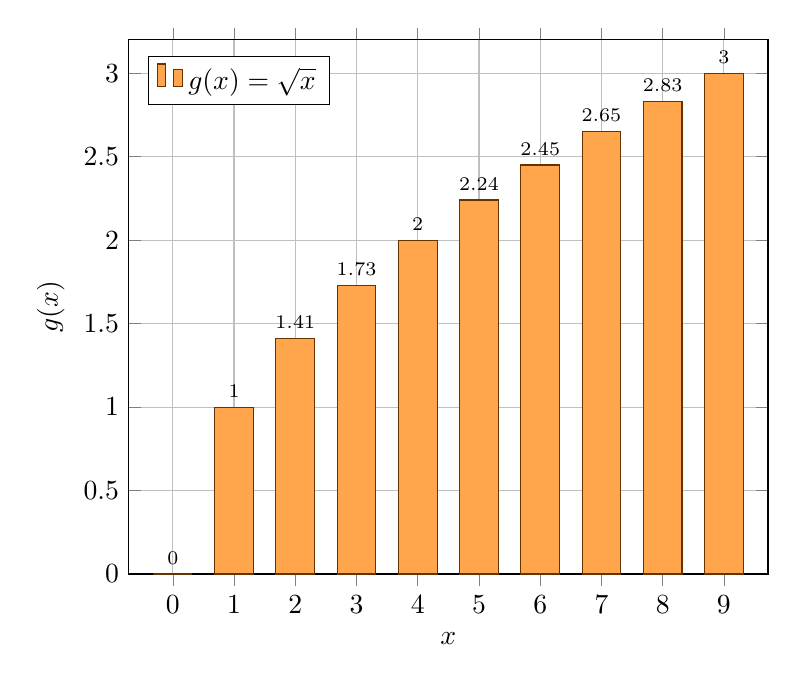
\begin{tikzpicture}
    \begin{axis}[
      width=0.8\textwidth,
      ybar,
      bar width=14pt,
      xlabel={$x$},
      ylabel={$g(x)$},
      ymin=0,
      ymax=3.2,
      symbolic x coords={0,1,2,3,4,5,6,7,8,9},
      xtick=data,
      enlarge x limits=0.08,
      grid=major,
      nodes near coords,
      every node near coord/.append style={font=\scriptsize},
      legend pos=north west
    ]
      \addplot[fill=orange!70, draw=orange!40!black] coordinates {
        (0,0)
        (1,1)
        (2,1.41)
        (3,1.73)
        (4,2)
        (5,2.24)
        (6,2.45)
        (7,2.65)
        (8,2.83)
        (9,3)
      };
      \addlegendentry{$g(x)=\sqrt{x}$}
    \end{axis}
  \end{tikzpicture}
  \caption{Przykładowy wykres słupkowy funkcji pierwiastkowej}
  \label{fig:wykres-slupkowy-pierwiastkowej}
\end{figure}

Przykładowy wykres funkcji sinus w przedziale \([0, 2\pi]\) przedstawiono na rysunku \ref{fig:wykres-sinusa}. Dla funkcji
\(h(x)=\sin(x)\) wartości okresowo zmieniają się od \(-1\) do \(1\), przyjmując zera w punktach \(0\), \(\pi\) oraz \(2\pi\).

\begin{figure}[!ht]
  \centering
  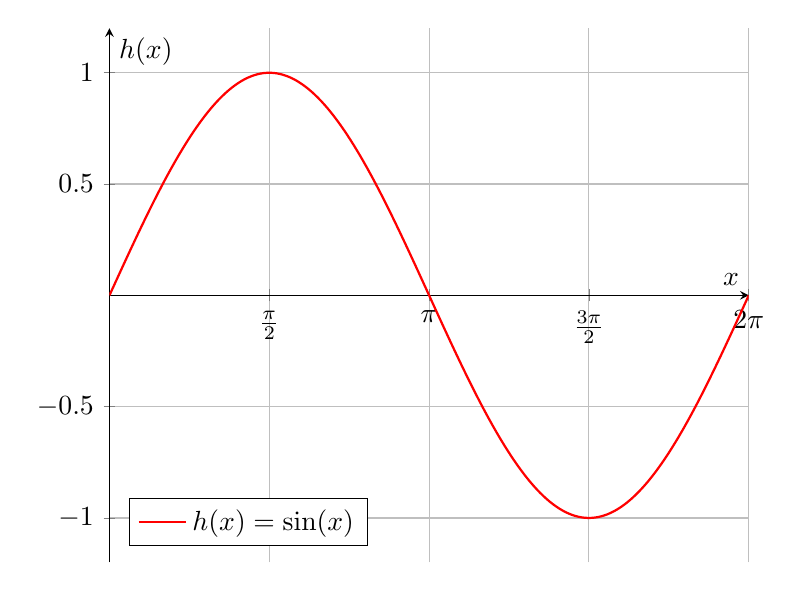
\begin{tikzpicture}
    \begin{axis}[
      width=0.8\textwidth,
      xlabel={$x$},
      ylabel={$h(x)$},
      grid=both,
      domain=0:2*pi,
      samples=200,
      axis lines=middle,
      ymin=-1.2,
      ymax=1.2,
      xtick={0,pi/2,pi,3*pi/2,2*pi},
      xticklabels={$0$, $\frac{\pi}{2}$, $\pi$, $\frac{3\pi}{2}$, $2\pi$},
      legend pos=south west
    ]
      \addplot[thick, red] {sin(deg(x))};
      \addlegendentry{$h(x)=\sin(x)$}
    \end{axis}
  \end{tikzpicture}
  \caption{Wykres funkcji sinus w przedziale od $0$ do $2\pi$}
  \label{fig:wykres-sinusa}
\end{figure}


\clearpage
\section{Schemat elektryczny prostownika}

Na rysunku \ref{fig:schemat-prostownika} przedstawiono przykładowy schemat jednofazowego prostownika mostkowego (mostek Graetza) z obciążeniem rezystancyjnym.

\begin{figure}[!ht]
  \centering
  \begin{tikzpicture}[american, scale=1]
    \draw
      (0,0) to[sV, l=$u_{we}(t)$] (0,4)
      (0,4) -- (2,4)
      (0,0) -- (2,0)

      (2,4) to[D, *-*, l=$D_1$] (4,6)
      (4,6) to[D, *-*, l=$D_2$] (6,4)
      (2,0) to[D, *-*, l_=$D_3$] (4,-2)
      (4,-2) to[D, *-*, l_=$D_4$] (6,0)

      (4,6) -- (8,6)
      (8,6) to[R, l=$R_{obc}$] (8,-2)
      (8,-2) -- (4,-2)

      (6,4) -- (8,4)
      (6,0) -- (8,0)
      (8,4) -- (8,6)
      (8,0) -- (8,-2);

    \draw (8,6) node[right] {$+$};
    \draw (8,-2) node[right] {$-$};
  \end{tikzpicture}
  \caption{Schemat elektryczny prostownika mostkowego}
  \label{fig:schemat-prostownika}
\end{figure}
